\documentclass[11pt]{article}
\usepackage[a4paper,margin=1.1in]{geometry}
\usepackage{fontspec}
\setmainfont{Georgia}
\usepackage{setspace}\setstretch{1.12}
\usepackage{indentfirst}
\emergencystretch=2em
\renewcommand{\labelitemii}{\textbullet}
\usepackage{titlesec}
\setcounter{secnumdepth}{2}
\titleformat{\section}{\large\bfseries}{\thesection}{0.6em}{}
\titlespacing*{\section}{0pt}{1.6em}{0.6em}
\titleformat{\subsection}{\normalsize\bfseries}{\thesubsection}{0.6em}{}
\titlespacing*{\subsection}{0pt}{1.2em}{0.4em}
\titleformat{\subsubsection}[runin]{\normalsize\itshape}{}{0pt}{}[.]
\titlespacing*{\subsubsection}{0pt}{0.8em}{0.5em}
\usepackage{xcolor}
\usepackage{amsmath,amssymb,amsthm,booktabs,array}
\usepackage{tikz}
\usetikzlibrary{arrows.meta,positioning,calc}
\usepackage{graphicx}
\newtheorem{proposition}{Proposition}
\newtheorem{lemma}{Lemma}
\usepackage[backend=biber,style=authoryear,maxcitenames=2,maxbibnames=6,giveninits=true,uniquename=false,uniquelist=false,doi=true,url=false,isbn=false]{biblatex}
\addbibresource{refs.bib}
\usepackage{hyperref}\hypersetup{colorlinks=true,linkcolor=black,citecolor=blue!50!black,urlcolor=blue!50!black}
\newcommand{\NUM}[1]{\textcolor{red!70!black}{\textbf{[NUM: #1]}}}
\newcommand{\REV}[1]{\textcolor{purple!70!black}{\textbf{[REV: #1]}}}
\newcommand{\HEDGE}[1]{\textcolor{green!40!black}{\textbf{[HEDGE: #1]}}}
\newcommand{\PRO}[1]{\textcolor{blue!55!black}{\textbf{[PRO: #1]}}}
\newcommand{\EX}[1]{\textcolor{orange!80!black}{\textbf{[EX: #1]}}}
\newcommand{\Q}[1]{\textcolor{violet!70!black}{\textbf{[QUOTE: #1]}}}
\title{How-possibly and how-actually:\\ what a resting-state manifold explains}
\author{P.~Mahon \\ \small Draft v3: the proof-like steps written out; numerical slots still marked. \\ \small Every sentence is a draft for rewrite.}
\date{17 November 2026}
\begin{document}
\maketitle

\section*{Opening}
\textcite{fousek2024} offer a mechanistic account of the brain's resting state: a network of bistable regions, coupled through a measured connectome and driven by noise, settles onto a low-dimensional manifold whose structured flow produces the dynamic functional connectivity, the co-activation events and the cascades seen in resting fMRI and EEG. I will ask what kind of explanation the paper gives, and whether its evidence supports that kind. I will argue three things. The paper supplies a \emph{how-possibly} explanation of its phenomena, in \textcite{craver2006}'s sense of a model that shows how a mechanism could produce them, and presents it as a \emph{how-actually} explanation, one that shows how the mechanism does. The strongest reply available to the authors relocates this problem rather than removing it. And, stated as what it is, the paper is the first half of a well-formed explanatory project whose second half is testable and untested. A how-possibly model is a precondition of a how-actually one, not a failed version of it: a mechanism whose output is nowhere near the data is not a candidate at all. The question is what, beyond nearness, is needed.

My answer has two parts, and they are the two conditions of one proposition. The statistics by which the paper selects its model each have a kernel: changes to a record that they cannot register; call that invariance. And the class of models over which the claim is made contains changes of mechanism that stay inside that kernel; call that equivariance. Where both hold, fit constrains nothing, and the mechanism is identified only up to what the statistic cannot see. In the terms of backward error analysis as Corless and Fillion present it \parencite{corless2016,fillion2014}, the paper establishes a backward error, the data are the exact output of a nearby model, and reports it as a forward error, a bound on which models the data admit. The gap between the two is the condition number of the statistic, and along the kernel it is infinite.

I hold the paper to its own standard of mechanistic explanation. I show that each statistic it selects by is blind to a class of changes in the record; that for the two statistics blind to order in time, every class of models the paper can be read as claiming over contains a change of generator inside or close to that blind class, exactly for the covariance statistic, to within a small measured distance for the histogram, and within the field's own criteria for the warranted rivals, so the fit cannot tell those generators apart; and that the one statistic which does see switching has no stated tolerance against which to read it. I grant the authors their strongest reply, that the warrant comes from the parts and not from the fit, and show that it narrows the class of rivals without closing it. I end with what the paper's own standard asks for next: tests it names and has not run.

\section{The explanandum: data and phenomena}
Definitions first. I will refer to the resting-state features the paper sets out to explain as `the phenomena', in the sense of \textcite{bogen1988}, to the network model as `the mechanism', and to the low-dimensional object the model produces as `the manifold'. By `data' I mean the recorded BOLD and EEG time series. By `phenomena' I mean, more precisely, the stable patterns extracted from data by a procedure: here, the fluidity of sliding-window functional connectivity, the share of variance carried by two principal components, and the statistics of high-amplitude co-activation events. A phenomenon is only as fine as the statistic that defines it.


\section{The explanatory claim and its standard}
The paper is explicit about what it wants. Earlier models, it says, ``leave a gap in the description of a mechanism''; to explain ``is thus not merely to redescribe one regularity \ldots\ as a series of several'', but to reveal ``the productive relation between causal activities linked to their constituent entities'' \parencite[Introduction]{fousek2024}. This is mechanistic explanation in the sense of \textcite{mdc2000} and \textcite{craver2007}: entities (regions, tracts, bistable populations) and activities (noise-driven switching between up and down states), organized so as to produce the phenomenon.

The standard carries its own tests.
\begin{enumerate}
\item \textcite{craver2006} distinguishes a \emph{how-possibly} model, which shows that a mechanism could produce the phenomenon, from a \emph{how-actually} model, which shows that it does; only the second explains, although the first is required for it.
\item The components of a how-actually model must be \emph{constitutively relevant}, which Craver cashes out as mutual manipulability: intervening on a part changes the whole, and intervening on the whole changes the part \parencite{craver2007}.
\end{enumerate}
In its Discussion the paper says that ``our goal here is not to generate in silico observables that are as close as possible to the empirical one'' \parencite[Discussion]{fousek2024}, while also using closeness to data as evidence, in the coincidence of the fluidity peak with the minimum of the histogram distance. It does not disclaim realism. It asserts a mechanism of the brain.

\section{The objection: underdetermination of the mechanism by the phenomena}
\subsection{The dart board}
Here is the objection in its plainest form. The phenomena of \S1 are coarse functionals of the data. Many generative hypotheses entail the same values of those functionals, and \S3.4 to \S3.6 say which, statistic by statistic.

I want to be precise about which underdetermination this is. It is not the Duhem--Quine kind, where any hypothesis can be saved by adjusting auxiliaries. It is \emph{contrastive}, in the sense \textcite{laudan1991} separate from holism: the evidence fails to discriminate the proposed mechanism from a wide class of alternatives that entail the same phenomena. The inference from ``the model produces the phenomena'' to ``the model's mechanism is the brain's'' is then an inference to \emph{an} explanation, not to the best \parencite{lipton2004}. In Craver's terms, a how-possibly model has been offered as how-actually. I will refer to this as `the dart-board objection': throw a dart at the space of models and you hit one that reproduces the phenomena.

\subsection{Backward and forward error}
The same point can be put in the language of backward error analysis, which Fillion and Corless read as an epistemology of modelling and not only a tool for algorithms \parencite{fillion2014}; the numerical form below is Corless and Fillion's \parencite{corless2016}. Write $\Psi$ for the map that takes a parameter setting $\theta$ (coupling, noise, connectome, node regime) to the law of the BOLD record the model generates at that setting. Write $\varphi$ for the map that takes a BOLD record to the number or numbers that define a phenomenon: the fluidity index, or the explained-variance share. Write $\pi(\theta)$ for the part of $\theta$ that says which mechanism it is, the regime, the coupling structure, the noise law, as against the part that only tunes it. In symbols,
\begin{equation}
y \mapsto \varphi(y)\in\mathbb{R}^{k}, \qquad \theta \mapsto \varphi(\Psi(\theta)), \qquad \theta \mapsto \pi(\theta),
\label{eq:objects}
\end{equation}

The backward-error question, in the form \textcite{corless2016} give it after \textcite{wilkinson1963}, is whether the computed answer is the exact answer to a nearby problem. Here it is whether the data are the exact output of a nearby model, with distance measured by the statistic. Corless and Fillion's concluding gloss is the most charitable reading of the paper available: backward error analysis ``interprets the computed solution \ldots\ $z$ as the exact solution to just as good a model''. Whether the nearby model is just as good is the whole question. They add two cautions: (i) a residual can be zero and, if there are several solutions, one still needs a way to get the right one; (ii) a small residual is not enough without the sensitivity of the model to perturbation, ``even if $\Delta\equiv 0$''. Define
\begin{equation}
\beta(y)\;=\;\inf_{\theta}\,\bigl\|\varphi(\Psi(\theta))-\varphi(y)\bigr\|,
\qquad
A_{\varepsilon}\;=\;\bigl\{\theta \;\big|\; \|\varphi(\Psi(\theta))-\varphi(y)\|\le\varepsilon\bigr\}.
\label{eq:beta}
\end{equation}
The paper establishes that $\beta$ is small at its working point.

What how-actually requires is a bound on the \emph{forward} error $\delta$: the size of $A_\varepsilon$ in the coordinates that distinguish mechanisms. To first order, forward error is backward error times a condition number \parencite{higham2002,corless2016} (Figure~\ref{fig:bf}):
\begin{equation}
\delta(y)\;=\;\operatorname{diam}\,\pi\bigl(A_{\varepsilon}(y)\bigr)\;\le\;2\kappa\,\varepsilon,
\qquad
\kappa \;=\; 1\big/\sigma_{\min}\!\bigl(J_{\pi}\bigr),
\label{eq:forward}
\end{equation}
where $J_\pi$ is the Jacobian of $\varphi\circ\Psi$ in the mechanism coordinates after the tuning coordinates have been projected out (the Schur complement of the full Jacobian), since a move in $\pi$ can be compensated by a move in the tuning coordinates. The bound is local, and $A_\varepsilon$ need not be connected, which is caution (i) again. For models of this kind the singular values span many decades \parencite{gutenkunst2007,machta2013,transtrum2015}, so $\kappa$ is large along most directions, and disparate parameter sets yield the same activity \parencite{prinz2004}. Caution (i), several solutions and nothing to pick the right one, can be made exact in the vocabulary of identification theory \parencite{rothenberg1971}. Two parameter values are \emph{observationally equivalent} with respect to a statistic when they induce the same law of that statistic. A parameter direction is \emph{identified} only if no such equivalence runs along it.

\begin{figure}[htbp]\centering
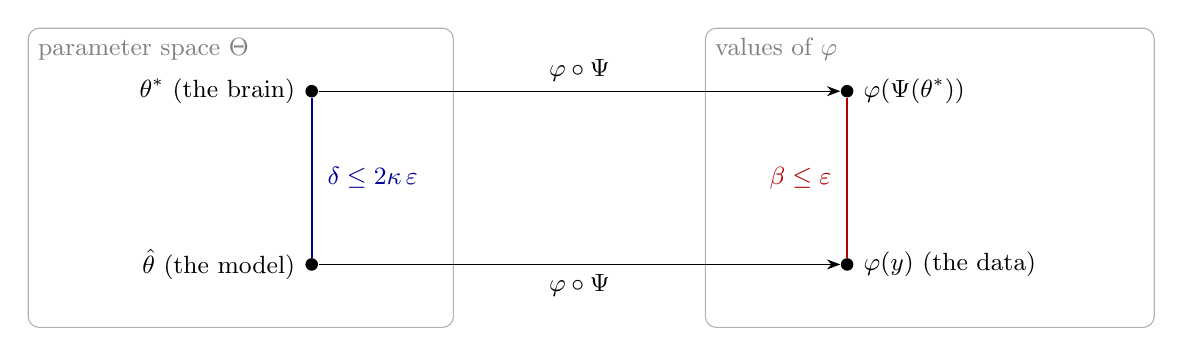
\begin{tikzpicture}[>=Stealth, font=\small]
  \draw[rounded corners, gray!60] (-2.0,-2.2) rectangle (3.4,1.6);
  \node[gray, anchor=north west] at (-2.0,1.6) {parameter space $\Theta$};
  \draw[rounded corners, gray!60] (6.6,-2.2) rectangle (12.3,1.6);
  \node[gray, anchor=north west] at (6.6,1.6) {values of $\varphi$};
  \node[circle,fill,inner sep=1.6pt,label=left:{$\theta^{*}$ (the brain)}] (ts) at (1.6,0.8) {};
  \node[circle,fill,inner sep=1.6pt,label=left:{$\hat\theta$ (the model)}] (th) at (1.6,-1.4) {};
  \node[circle,fill,inner sep=1.6pt,label=right:{$\varphi(\Psi(\theta^{*}))$}] (ps) at (8.4,0.8) {};
  \node[circle,fill,inner sep=1.6pt,label=right:{$\varphi(y)$ (the data)}] (py) at (8.4,-1.4) {};
  \draw[->] (ts) -- node[above]{$\varphi\circ\Psi$} (ps);
  \draw[->] (th) -- node[below]{$\varphi\circ\Psi$} (py);
  \draw[thick, red!70!black] (ps) -- node[left, xshift=-2pt]{$\beta\le\varepsilon$} (py);
  \draw[thick, blue!60!black] (ts) -- node[right, xshift=2pt]{$\delta\le 2\kappa\,\varepsilon$} (th);
\end{tikzpicture}
\caption{Backward and forward error, in the layout of the commutative diagram of \textcite[\S2]{corless2016} (cf.\ \textcite[Fig.~1.1]{higham2002}), with the labels of \eqref{eq:objects}. Left: parameter space $\Theta$, with the brain's parameters $\theta^{*}$ and the model's $\hat\theta$. Right: the values of the statistic, with the image of each under $\varphi\circ\Psi$ and the observed value $\varphi(y)$. The red segment is the backward error $\beta$ of \eqref{eq:beta}, measured on the right; the blue segment is the forward error $\delta$, measured on the left, with the bound $2\kappa\varepsilon$ of \eqref{eq:forward}.}
\label{fig:bf}
\end{figure}



\subsection{Non-identification along the kernel}
\begin{proposition}[non-identification along the kernel]
Let $K$ be a group of measurable transformations of the data, and let $\theta+\mathbb{R}v\subset\Theta$. Suppose (i) the statistic is \emph{invariant}: $\varphi\circ g=\varphi$ for every $g\in K$; and (ii) the model is \emph{equivariant along the direction $v$}: for every $t$, $\Psi(\theta+tv)=g_{t*}\Psi(\theta)$ for some $g_t\in K$, where $g_{t*}$ is the pushforward of a law by $g_t$ ($g_t$ may be drawn at random, independently of the record, since (i) holds record by record). Write $p_\theta$ for the law of $\varphi$ under $\Psi(\theta)$ and $\varphi(\Psi(\theta))$ for a fixed functional of it, its mean say. Then every $\theta+tv$ is observationally equivalent to $\theta$ with respect to $\varphi$, so $\theta$ is not identified along $v$, locally or globally; if the family $\{p_\theta\}$ is differentiable in quadratic mean at $\theta$, its information matrix is singular along $v$; and if $\theta\in A_\varepsilon(y)$ then $\theta+\mathbb{R}v\subset A_\varepsilon(y)$.
\end{proposition}
\begin{proof}
For any bounded $h$, by the change of variables for the pushforward and condition (i),
\[
\mathbb{E}_{\theta+tv}\bigl[h(\varphi)\bigr]=\int h\circ\varphi\;d\bigl(g_{t*}\Psi(\theta)\bigr)=\int h\circ\varphi\circ g_t\;d\Psi(\theta)=\mathbb{E}_{\theta}\bigl[h(\varphi)\bigr],
\]
so $p_{\theta+tv}=p_\theta$ for every $t$. Every neighbourhood of $\theta$ therefore contains points observationally equivalent to it, which is local non-identification by definition, and global non-identification since $t$ is unrestricted; this is the situation Rothenberg's rank condition describes \parencite{rothenberg1971}. Under differentiability in quadratic mean, $\sqrt{p_{\theta+tv}}=\sqrt{p_\theta}$ in $L^2$, so the $L^2$-derivative along $v$ vanishes and
\[
v^{\top}I(\theta)\,v=\mathbb{E}_\theta\bigl[(\partial_v\log p_\theta)^2\bigr]=0.
\]
Finally, if $\theta\in A_\varepsilon(y)$, then for every $t$
\[
\|\varphi(\Psi(\theta+tv))-\varphi(y)\|=\|\varphi(\Psi(\theta))-\varphi(y)\|\le\varepsilon,
\]
so $\theta+\mathbb{R}v\subset A_\varepsilon(y)$.
\end{proof}
The pair is the standard one in the theory of invariance \parencite[ch.~6]{lehmann2005}: a group $K$ acting on the sample space, with an induced action $\bar g$ on the parameter space, such that
\[
\varphi\circ g=\varphi \quad\text{(invariant statistic)}, \qquad g_{*}\Psi(\theta)=\Psi(\bar g\,\theta) \quad\text{(equivariant model)},
\]
and here $\bar g_t\,\theta=\theta+tv$ (Figure~\ref{fig:prop}).

\begin{figure}[htbp]\centering
\resizebox{\textwidth}{!}{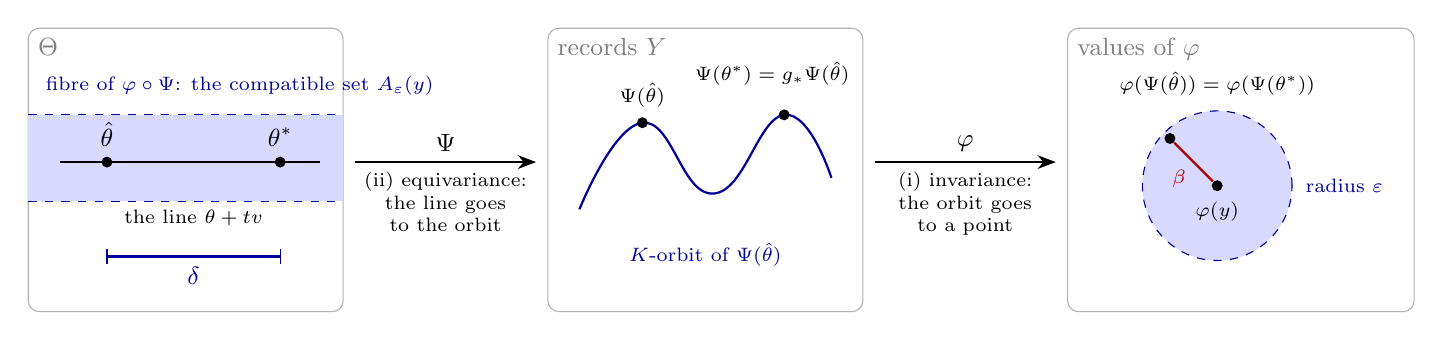
\begin{tikzpicture}[>=Stealth, font=\small]
  % ---- Theta ----
  \draw[rounded corners, gray!60] (0,0) rectangle (4.0,3.6);
  \node[gray, anchor=north west] at (0,3.6) {$\Theta$};
  \fill[blue!15] (0,1.4) rectangle (4.0,2.5);
  \draw[blue!60!black, dashed] (0,1.4) -- (4.0,1.4); \draw[blue!60!black, dashed] (0,2.5) -- (4.0,2.5);
  \node[blue!60!black, anchor=south west, font=\scriptsize] at (0.1,2.62) {fibre of $\varphi\circ\Psi$: the compatible set $A_\varepsilon(y)$};
  \draw[thick] (0.4,1.9) -- (3.7,1.9);
  \node[anchor=north, font=\scriptsize] at (2.1,1.42) {the line $\theta+tv$};
  \node[circle,fill,inner sep=1.4pt,label={[font=\small]above:$\hat\theta$}] (th) at (1.0,1.9) {};
  \node[circle,fill,inner sep=1.4pt,label={[font=\small]above:$\theta^{*}$}] (ts) at (3.2,1.9) {};
  \draw[thick, blue!60!black] (1.0,0.7) -- node[below]{$\delta$} (3.2,0.7);
  \draw[blue!60!black] (1.0,0.6) -- (1.0,0.8); \draw[blue!60!black] (3.2,0.6) -- (3.2,0.8);
  % ---- Y ----
  \draw[rounded corners, gray!60] (6.6,0) rectangle (10.6,3.6);
  \node[gray, anchor=north west] at (6.6,3.6) {records $Y$};
  \draw[thick, blue!60!black] plot[smooth, tension=0.8] coordinates {(7.0,1.3) (7.8,2.4) (8.7,1.5) (9.6,2.5) (10.2,1.7)};
  \node[blue!60!black, anchor=north, font=\scriptsize] at (8.6,1.0) {$K$-orbit of $\Psi(\hat\theta)$};
  \node[circle,fill,inner sep=1.4pt,label={[font=\scriptsize]above:$\Psi(\hat\theta)$}] (yh) at (7.8,2.4) {};
  \node[circle,fill,inner sep=1.4pt] (ys) at (9.6,2.5) {};
  \node[anchor=south, font=\scriptsize] at (9.45,2.75) {$\Psi(\theta^{*})=g_*\Psi(\hat\theta)$};
  % ---- values ----
  \draw[rounded corners, gray!60] (13.2,0) rectangle (17.6,3.6);
  \node[gray, anchor=north west] at (13.2,3.6) {values of $\varphi$};
  \draw[blue!60!black, dashed, fill=blue!15] (15.1,1.6) circle (0.95);
  \node[blue!60!black, anchor=west, font=\scriptsize] at (16.1,1.6) {radius $\varepsilon$};
  \node[circle,fill,inner sep=1.4pt,label={[font=\scriptsize]below:$\varphi(y)$}] (py) at (15.1,1.6) {};
  \node[circle,fill,inner sep=1.4pt] (pp) at (14.5,2.2) {};
  \node[anchor=south, font=\scriptsize] at (15.1,2.62) {$\varphi(\Psi(\hat\theta))=\varphi(\Psi(\theta^{*}))$};
  \draw[thick, red!70!black] (py) -- node[below left, xshift=1pt, yshift=1pt, font=\scriptsize]{$\beta$} (pp);
  % ---- arrows between boxes ----
  \draw[->, thick] (4.15,1.9) -- node[above]{$\Psi$} node[below, font=\scriptsize, align=center, text width=2.3cm]{(ii) equivariance: the line goes to the orbit} (6.45,1.9);
  \draw[->, thick] (10.75,1.9) -- node[above]{$\varphi$} node[below, font=\scriptsize, align=center, text width=2.3cm]{(i) invariance: the orbit goes to a point} (13.05,1.9);
\end{tikzpicture}}
\caption{The two conditions of the Proposition, each in its own space, and the fibre they produce. Left: parameter space $\Theta$, with the line $\theta+tv$ through the model's parameters $\hat\theta$ and the brain's $\theta^{*}$. Middle: the space of records $Y$, with the $K$-orbit of the model's law $\Psi(\hat\theta)$; under condition (ii), equivariance, $\Psi$ carries the line onto the orbit, so $\Psi(\theta^{*})=g_*\Psi(\hat\theta)$ for some $g\in K$. Right: the values of the statistic; under condition (i), invariance, $\varphi$ is constant on the orbit, so the whole line has one image, which lies within $\varepsilon$ of the observed value $\varphi(y)$. The red segment is the backward error $\beta$ of \eqref{eq:beta}, the same for every point of the line. The shaded strip on the left is the preimage of the $\varepsilon$-ball, the compatible set $A_\varepsilon(y)$, which contains the whole line; the blue segment is the forward error $\delta$ of \eqref{eq:forward} between $\hat\theta$ and $\theta^{*}$, unbounded along $v$. The layout extends the commutative diagram of \textcite[\S2]{corless2016}, after \textcite[Fig.~1.1]{higham2002}, by one box.}
\label{fig:prop}
\end{figure}

The Proposition has two conditions. Invariance says there are changes to a record that the statistic does not notice; equivariance says there are changes to the model that produce exactly such changes to the record.
\begin{enumerate}
\item[(i)] \emph{Invariance.} The first concerns the statistic the authors chose, and is settled from the definitions. (Notation as in Appendix~A: $C(y)$ is the sample covariance, $D_{ij}$ the correlation between the connectivity vectors of windows $i$ and $j$, $W$ the window length.) Each statistic fixes its own group $K$:
  \begin{itemize}
  \item[(a)] The explained-variance share $\varphi_a$ (\S3.4) depends on the record only through the eigenvalues of $C(y)$, so
  $K_a=\{g:\ C(gy)=C(y)\ \text{for every } y\}$: the transformations that keep every record's sample covariance. The phase maps of Appendix~A and the permutations of the samples belong to it.
  \item[(b)] The histogram statistic $\varphi_b$ (the KS distance on the centred $D_{ij}$, $i<j$; \S3.5) depends only on the multiset $\{D_{ij}\}$, so as a function of the window sequence it is unchanged by every reordering of the windows: dwell times and the order of recurrences are invisible to it. On records the windows overlap, and only time reversal realises a reordering, so $K_b=\{\text{identity},\ \text{reversal}\}$; the order-blindness is a property of the statistic, not a symmetry a generator can exploit.
  \item[(c)] The fluidity index $\varphi_c=\operatorname{Var}\{D_{ij}\mid |i-j|\ge W\}$ (\S3.6) depends only on the multiset over unordered pairs at least a window apart; with more than $2W$ windows the only reorderings that preserve that pair set are the identity and reversal, so $K_c=\{\text{identity},\ \text{reversal}\}$ as well. (Per-region positive affine maps also leave $\varphi_b$ and $\varphi_c$ unchanged, being built from correlations; they are not used below.)
  \end{itemize}
\item[(ii)] \emph{Equivariance.} The second concerns the model class over which the claim is made: whether some change of parameters is intertwined, through $\Psi$, with an element of $K$. That depends on the class, and the paper can be read over three, nested:
  \begin{itemize}
  \item[$\Theta_1$] the paper's own grid, $\{(G,\sigma)\}$, with the connectome $W$ and the node model fixed;
  \item[$\Theta_2$] $\Theta_1$ together with a regime coordinate $r\in R$, $R=\{$bistable, near-Hopf, excitable, metastable$\}$ on the same connectome: the class the authors' reply in \S4 will name, mechanisms with independently warranted parts. One member of $R$ is of our own construction, a two-state reduction of the node (each region up or down, flipping at the full model's own rates) on the same connectome; it is the only witness below that is not borrowed;
  \item[$\Theta_3$] every generator reachable from the model along a path of transformations in $K$: for the phase map of Appendix~A, the path $\gamma(s)$, $s\in[0,1]$, whose law at $s$ is that of $g_{s\Phi}Y$ with $Y\sim\Psi(\theta)$, from the model at $s=0$ to its phase-randomised surrogate at $s=1$. It is the smallest class in which the Proposition's line exists, with direction $\gamma'(0)$; so $\Theta_1\subset\Theta_2\subset\Theta_3$.
  \end{itemize}
\end{enumerate}
The next three subsections take the statistics (a) to (c) in turn, and each is set against the three classes, so the whole is a grid of nine cases. Each subsection has the same two steps. Under \emph{condition (i), invariance}, I say what $K$ is. Under \emph{condition (ii), equivariance}, I ask, for $\Theta_1$, $\Theta_2$ and $\Theta_3$ in turn, whether some direction $v$ in the class is intertwined through $\Psi$ with an element of $K$. Each case is written in three slots, in the order backward error analysis prescribes. \emph{Direction}: which parameter $v$ moves. \emph{Backward error}: how far the statistic moves along it,
\begin{equation}
\beta_v(\theta)\;=\;\sup_{t}\,\bigl\|\varphi(\Psi(\theta+tv))-\varphi(\Psi(\theta))\bigr\|,
\label{eq:betav}
\end{equation}
graded \emph{exact} ($\beta_v=0$: a symmetry, and the Proposition applies), \emph{approximate} ($0<\beta_v\le\varepsilon$: the direction lies in $A_\varepsilon(y)$ but not in $A_0(y)$) or \emph{none} ($\beta_v>\varepsilon$: the statistic identifies $v$ to within $\varepsilon$), with the proof or the number that establishes the grade; I write $A_\varepsilon(y)$ with the data shown, because a witness found against one dataset is not yet a witness against another. \emph{Forward error}: what the grade does to $\kappa$ in \eqref{eq:forward}, and which coordinate of $\pi$ is therefore identified or not.

\subsection{The explained-variance share}
The paper reports the variance explained by the first two principal components of the regional time series; everything here holds for any number of components, and for any statistic that is a function of the sample covariance alone.

\subsubsection{Condition (i): invariance}
$\varphi_a\circ g=\varphi_a$ for every $g\in K_a$: the share is a function of the eigenvalues of $C(y)$ and of nothing else. With $\lambda_1\ge\dots\ge\lambda_N$ the eigenvalues of $C(y)$, $\varphi_a(y)=(\lambda_1+\lambda_2)/\sum_i\lambda_i$, and every $g\in K_a$ fixes $C(y)$; so $\varphi_a(gy)=\varphi_a(y)$ for every $g\in K_a$.

\subsubsection{Condition (ii): equivariance}
\begin{itemize}
\item[$\Theta_1$]
  \begin{itemize}
  \item \emph{Direction}: $v=\partial_G$, the coupling, with $W$ and the node model fixed.
  \item \emph{Backward error}: $\beta_v>0$, since moving $G$ moves $C(y)$; but $\beta_v\le\varepsilon$ across the band in $G$ that the paper's own sweep displays: approximate. In the reimplementation's sweep at $\sigma=0.18$ the up-containing switching states occupy $G\approx0.9$--$1.0$ of a range 0.3--1.6, about a tenth of it, and the transition regime occupies one cell of twenty-one swept at $\sigma\ge0.20$; below the band the network is all-down and above it locked up. (Where the record is nearly constant the switching index is inflated by the correlation of near-constant signals and is not used to delimit the band.)
  \item \emph{Forward error}: $\kappa$ finite but large along $G$; the working point is a band, not a point.
  \end{itemize}
\item[$\Theta_2$]
  \begin{itemize}
  \item \emph{Direction}: $v=\partial_r$, the regime coordinate.
  \item \emph{Backward error}: the published witnesses are covariance-level, which is the level this statistic reads. On the same kind of connectome a linear spatial autoregressive model predicts static functional connectivity as well as or better than seven nonlinear network models \parencite{messe2014,messe2015}, and across 700 HCP subjects linear autoregressive models fit macroscopic resting dynamics best on prediction, complexity and residual structure \parencite{nozari2024}. A statistic that is a function of the covariance cannot separate those generators from this one. The studies report correlations and model comparisons, not a tolerance, so the grade is approximate relative to their own criteria and their own data, carried to $y$ by the paper's implicit pooling across datasets. The two-state reduction of our own reaches the model's all-down and mostly-up states and not its mixed state. In the mostly-up state at $G=1.0$ it does not: two components carry 0.29--0.32 of its variance against the model's 0.50--0.51. At the transition regime, from the start that produces global excursions, it does: 0.98 against 0.98.
  \item \emph{Forward error}: $\kappa$ large along $r$; the regime, and the linear-against-nonlinear distinction with it, is not identified by $\varphi_a$ at the field's own criteria.
  \end{itemize}
\item[$\Theta_3$]
  \begin{itemize}
  \item \emph{Direction}: the path $\gamma$ from the model to its phase-randomised surrogate (Appendix~A): the record with the same periodogram, hence the same sample covariance, and randomised phases.
  \item \emph{Backward error}: $\beta_v=0$ along $\gamma$: exact. (Lemma~\ref{lem:phase}: the phase map fixes every entry of the cross-periodogram, hence $C(y)$, so $g_\phi\in K_a$ for every $\phi$.)
  \item \emph{Forward error}: $\kappa=\infty$ along $\gamma$; the coordinate that separates ``bistable network'' from ``a stationary surrogate of itself with no mechanism'' is not identified at any tolerance, and the Proposition applies verbatim.
  \end{itemize}
\end{itemize}

\subsection{The histogram statistic}
The paper selects its working point by the distance between the histogram of window-pair correlations in the model and in an empirical session.
\subsubsection{Condition (i): invariance}
As a function of the window sequence, $\varphi_b$ is unchanged by any permutation $\sigma$ of the window indices: $\sigma$ sends $D_{ij}$ to $D_{\sigma(i)\sigma(j)}$, a bijection of the index pairs, so the multiset $\{D_{ij}: i<j\}$, its centred empirical distribution and the KS distance to any fixed reference are unchanged. On records, with 60\,s windows at 2\,s steps, consecutive windows share almost all their samples, and no map of the record realises a reordering of the windows other than time reversal. So the order-blindness is real, and is why the statistic cannot see switching, but $K_b$ as a group acting on data is $\{\text{identity},\ \text{reversal}\}$, and a generator cannot exploit it directly.

\subsubsection{Condition (ii): equivariance}
\begin{itemize}
\item[$\Theta_1$]
  \begin{itemize}
  \item \emph{Direction}: $v=\partial_\sigma$ at fixed $G$ inside the band.
  \item \emph{Backward error}: $\beta_v\le\varepsilon$ over a range of $\sigma$, since the multiset of correlations changes slowly there: approximate. Measured as the KS distance between the histograms of neighbouring $\sigma$ at fixed $G$: 0.05--0.19 per step of 0.02--0.03 within a regime, against a seed-to-seed floor of 0.06--0.10 at fixed parameters, and 0.41 across the regime boundary at $G=1.05$. So within a regime the histogram moves along $\sigma$ by about the sampling spread, and the selected point is a shallow valley; the valley ends where the regime does.
  \item \emph{Forward error}: $\kappa$ finite but large along $\sigma$; the selected point is the bottom of a shallow valley.
  \end{itemize}
\item[$\Theta_2$]
  \begin{itemize}
  \item \emph{Direction}: $v=\partial_r$, as for the share.
  \item \emph{Backward error}: two kinds of witness, neither with a tolerance. For a different regime on the same connectome: a Stuart--Landau network at the edge of its Hopf bifurcation minimises the KS distance between model and empirical FCD histograms on 24 subjects \parencite{deco2017}, with the value to be read from its figures. For stationary generators with the data's spectra: shared-phase phase randomisation and a multivariate AR(1) reproduce the per-edge sliding-window variance (about 0.6\,\% of edges rejected at FDR 0.05) and the coherence of the window correlations \parencite{liegeois2017}; single-session non-rejection of the same null is a low-powered result rather than a match \parencite{hindriks2016}; and an i.i.d.\ Gaussian null with the covariance alone reproduces the spatial structure of co-activation events but not their timing \parencite{novelli2022}. On the other side, in the one study that compared regimes on FCD directly, only nodes given local bistability switched and the linear model failed \parencite{hansen2015}. So: approximate on the field's evidence, resting on one Hopf-edge study and the stationary nulls, carried to $y$ by the paper's implicit pooling across datasets. The two-state reduction is again the one witness in hand. In the mostly-up state the two-state reduction's histogram lies at KS 0.12--0.16 from the model's, within about a factor of two of the seed-to-seed floor; at the transition regime it lies at 0.36--0.42, far outside it. The histogram separates this rival where the share and the fluidity index do not.
  \item \emph{Forward error}: $\kappa$ large along the stationary direction; along the regime coordinate the field's evidence is thin and divided.
  \end{itemize}
\item[$\Theta_3$]
  \begin{itemize}
  \item \emph{Direction}: the path $\gamma$ from the model to its phase-randomised surrogate, as for the share.
  \item \emph{Backward error}: $\beta_v>0$ but small: the surrogate keeps the covariance and the spectra and changes the histogram of window-pair correlations by a KS distance that is a number. In the single-basin states that distance is 0.04--0.15; in the transition regime it is 0.15--0.29 against the phase surrogate and 0.15--0.22 against the AR(1) null (twenty of each, two records). Approximate in the single-basin states, where the published counterpart is \textcite{liegeois2017}; in the transition regime the histogram registers the switching, through the bimodality of the window correlations rather than their order.
  \item \emph{Forward error}: $\kappa$ large along $\gamma$; the order of recurrences is identified by $\varphi_b$ only to within that KS tolerance. The statistic chosen to locate switching is nearly blind to the one thing switching is, order in time.
  \end{itemize}
\end{itemize}

\subsection{The fluidity index}
The fluidity index is the paper's measure of switching: recurrences of a connectivity pattern raise it and a drifting pattern lowers it. It peaks in the same band of $G$ as the explained-variance share, and the two peaks together locate the working point. Every number below is tied to a collective state. At the paper's coupling the reimplementation settles into single-basin states (all-down; a partial pattern with local switching; mostly-up); the paper's kind of regime, a low-activity state with repeated global high-activity intervals, appears at $G=1.05$, $\sigma=0.30$: six to eight transitions in ten minutes, high intervals of 10--13\,s, low intervals of about two minutes, in both seeds run (Figure~\ref{fig:f2}). It is more globally synchronised than the paper's working point (two components carry 0.98 of the variance against their 0.41), so the numbers from it are the paper's kind of regime at a stronger collective mode, and are reported for both regimes.


\begin{figure}[htbp]\centering
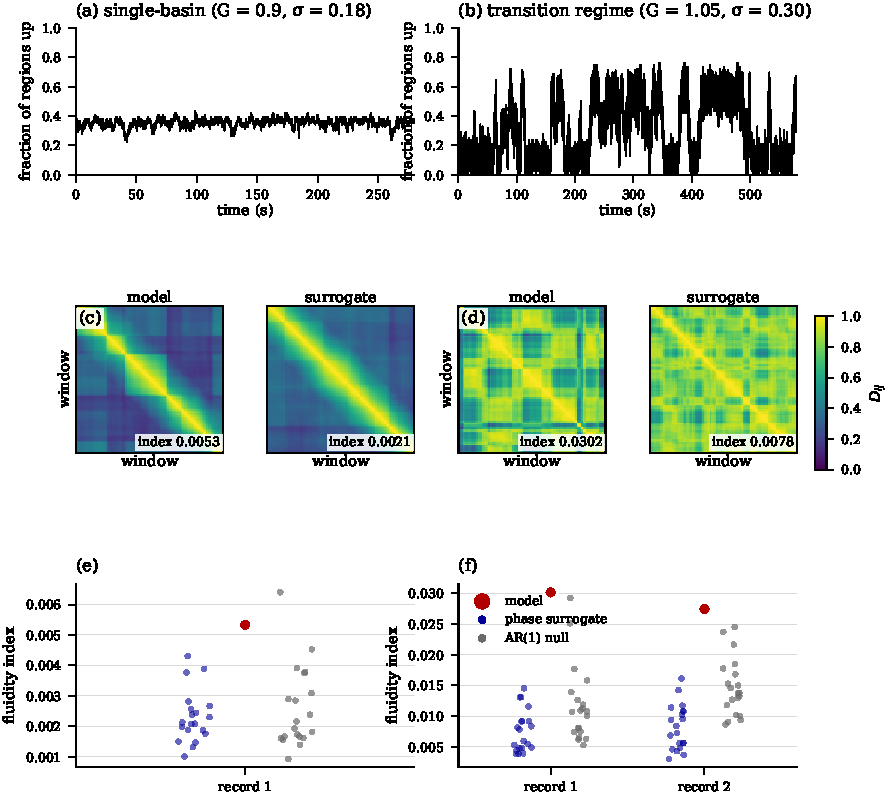
\includegraphics[width=\textwidth]{fig_f2.pdf}
\caption{In the single-basin regime a stationary null reproduces the order-blind statistics; in the transition regime the histogram and the fluidity index both separate the model from its null. Left column: the single-basin ``mixed'' state at $G=0.9$, $\sigma=0.18$; right column: the transition regime at $G=1.05$, $\sigma=0.30$. (a, b) Fraction of regions in the up state against time, one record each. (c, d) The window-correlation matrix $D_{ij}$ (60\,s windows, 2\,s steps) for the model record and for the phase-randomised surrogate of it whose index lies nearest the median of twenty; the number in each panel is that record's fluidity index; colour scale from 0 (dark) to 1 (light). (e, f) The fluidity index of each model record (large mark) against twenty phase-randomised surrogates (blue) and twenty realisations of a multivariate AR(1) fitted to the record (grey). Vertical scales differ between (e) and (f).}
\label{fig:f2}
\end{figure}

\subsubsection{Condition (i): invariance}
$\varphi_c\circ g=\varphi_c$ for $g\in K_c=\{\text{identity},\ \text{reversal}\}$, so the Proposition gives nothing here that reversal does not give, and reversal preserves dwell times. The variance is taken over the multiset $\{D_{ij}: |i-j|\ge W\}$; with more than $2W$ windows no other reordering preserves that pair set.

\subsubsection{Condition (ii): equivariance, by another route}
The case is made not by a symmetry but by a null. For any stationary record the index is positive, because windowed correlations are noisy estimates with correlated errors; its value under the null is what the phase-randomised surrogate of the model's own record measures exactly, and I write $s_0$ for that surrogate value. Lemma~\ref{lem:floor} (Appendix~A) explains its order of magnitude, under assumptions it states, as roughly one over the effective number of independent connectivity entries; it is an explanation, not a bound.
\begin{itemize}
\item[$\Theta_1$]
  \begin{itemize}
  \item \emph{Direction}: $v=\partial_G$ within the band.
  \item \emph{Backward error}: $\beta_v>0$; the index rises with $G$ as switching increases. What is missing is the $\varepsilon$ against which to grade it, and the null supplies one: $\varepsilon=s_0$, the index of the stationary surrogate with the model's own covariance and spectra. By surrogate, $s_0$ is 0.0014--0.0023 in the single-basin states and 0.008 (phase) to 0.012--0.015 (AR) in the transition regime; Lemma~\ref{lem:floor}'s weak-connectivity estimate overshoots the single-basin values by a factor of two to four.
  \item \emph{Forward error}: $\kappa$ finite; $\varphi_c$ identifies $G$ within the band to within $s_0$, and $s_0$ is the tolerance that \S7 asks the authors to report.
  \end{itemize}
\item[$\Theta_2$]
  \begin{itemize}
  \item \emph{Direction}: $v=\partial_r$.
  \item \emph{Backward error}: no witness exists either way; the Hopf-edge network of \textcite{deco2017} was scored on metastability and on the KS distance, not on this index, and whether $\|\varphi_c(\Psi(\theta_r))-\varphi_c(y)\|\le s_0$ for any $r\ne$ bistable is a number. No near-Hopf or metastable network has been run on this connectome. The two-state reduction is the one rival in hand. In the mostly-up state its index is 0.0006--0.0011 against the model's 0.0011--0.0028. At the transition regime, with hazards fitted from the model's own records, it attains the model's value from one start of three (0.0302 against 0.0302, with global excursions, two transitions in ten minutes to the model's six to eight) and stays in the low state from the other two. One rival of a different mechanism therefore attains the paper's fluidity index at its own kind of regime.
  \item \emph{Forward error}: undetermined until that number is in hand. The index separates the model from linear stationary nulls, so whether a rival mechanism on the same connectome attains the paper's value is what decides whether it identifies the regime. One does: the two-state reduction, from one start, attains it exactly. So $\varphi_c$ does not identify the regime against that rival, and the statistic that does is the histogram. Rivals of the published kinds, near-Hopf and metastable, have not been run on this connectome.
  \end{itemize}
\item[$\Theta_3$]
  \begin{itemize}
  \item \emph{Direction}: the path $\gamma$ to the phase-randomised surrogate, whose maps are not in $K_c$.
  \item \emph{Backward error}: not zero, and the comparison is a test rather than a distance along a line: the model's $\varphi_c$ against the distribution of $\varphi_c$ over surrogates of its own record. In the transition regime the model's index is 0.028--0.030 against 0.008 (phase) and 0.012--0.015 (AR): rank 21 of 21 under both nulls, in both records. In the single-basin ``mixed'' state the same holds (0.0053 and 0.0074 against 0.002); in the mostly-up state the null attains it.
  \item \emph{Forward error}: in the regime that matters, the model's value lies well outside its stationary null, so $\varphi_c$ does separate the model from that null, by a factor of two to four, and so does $\varphi_b$. How far that narrows $\pi$ among mechanisms is not computed here; it is the question of the $\Theta_2$ cell.
  \end{itemize}
\end{itemize}

\begin{table}[htbp]\centering\small
\caption{Grade of the backward error along each direction, by statistic and model class, and what establishes it. Rows: the three selection statistics (a)--(c). Columns: the three classes $\Theta_1\subset\Theta_2\subset\Theta_3$. Each cell gives the grade of $\beta_v$ along the direction treated in the corresponding case of \S3.4--\S3.6 and the kind of support it rests on. Grades: $0$ exact ($\beta_v=0$, $\kappa=\infty$); $\approx$ approximate ($\beta_v\le\varepsilon$); $G$ the statistic identifies the coupling to within the null value $s_0$; sep., the model's value lies outside its surrogate distribution; $?$ open. $^{\dagger}$In the transition regime; in the single-basin states the histogram is approximate and the fluidity index is attained in one state of three. $^{\ddagger}$Attained by the two-state reduction, one rival of our own; rivals of the published kinds not run. Support: P a proof in the text; C witnesses cited from the literature; N a number from the reimplementation.}
\label{tab:grid}
\renewcommand{\arraystretch}{1.25}
\begin{tabular}{@{}l ccc@{}}
\toprule
 & $\Theta_1$ grid $(G,\sigma)$ & $\Theta_2$ warranted mechanisms & $\Theta_3$ all generators \\
\midrule
(a) explained-variance share & $\approx$\ \ N & $\approx$\ \ C & $0$\ \ P \\
(b) histogram statistic      & $\approx$\ \ N & $\approx$\ \ C & $\approx$\ \ N$^{\dagger}$ \\
(c) fluidity index           & $G$\ \ N\ \ ($\varepsilon=s_0$) & $\approx$\ \ N$^{\ddagger}$ & sep.\ \ N$^{\dagger}$ \\
\bottomrule
\end{tabular}
\end{table}

By \eqref{eq:forward} (Table~\ref{tab:grid}), the fit constrains the coupling $G$ to a band, and nothing else that $\pi$ records: along the path to the model's own stationary surrogate $\delta$ is unbounded for the covariance statistic at every $\varepsilon$ and bounded only by a small measured tolerance for the histogram, along the regime coordinate it spans $R$ at the field's own criteria; the fluidity index and, in the transition regime, the histogram narrow it on the model side, against stationary nulls, and the open question is whether they narrow it against rival mechanisms. The Proposition does not say that the statistics register nothing; it says what they cannot register, and the paper's claim is made over exactly those coordinates.

The distinction is not new under other names. It is the econometrician's distinction between an identified set and point identification \parencite{koopmans1950,manski2003}; $A_0$ is Manski's identified set, and Manski himself has recently connected partial identification to underdetermination \parencite{manski2026}. Craver's distinction belongs beside it.

\section{On behalf of the authors: constitutive warrant}
On behalf of the authors one could reply as follows, and I think this is the strongest reply available. It has four parts.
\begin{enumerate}
\item[R1] \emph{The warrant comes from the parts, not from the fit.} The phenomena were never the warrant for the mechanism; they are the explanandum. The warrant comes from the independent evidence for the components, in the manner of \textcite{glymour1980}'s bootstrapping, or, in the numerical idiom, a \emph{structured} backward error in which the measured components are pinned and only the unmeasured ones may vary (Appendix~A): the connectome is measured, not fitted; the node model is derived exactly from spiking neurons \parencite{montbrio2015}; and bistability of single-region activation is supported by energy-landscape fits of resting data \parencite[refs 39--41 therein, Watanabe et al.\ 2013, 2014 and Gu et al.\ 2018]{fousek2024}.
\item[R2] \emph{Constitutive relevance is shown by manipulation.} Sweep the coupling and the phenomena come and go; replace the connectome with an all-to-all network and they vanish.
\item[R3] \emph{The contrast class of \S3 is mis-specified.} A stationary Gaussian process is a \emph{phenomenal} model in Craver's own sense, his Ptolemaic case: descriptively adequate and explanatorily empty, because it posits no components \parencite{craver2006}. It cannot compete with a mechanism, so it cannot underdetermine one. The relevant contrast class is mechanisms with independently warranted parts, $\Theta_2$.
\item[R4] \emph{The manifold earns its keep by prediction.} It is not a fitted object but a representational bridge between the parts and the phenomena, and it yields predictions outside the phenomena used for selection: the up-state frequency should rise with a region's in-strength; the time spent in cascades should fall along the cortical hierarchy; each subject's connectome should fix that subject's working point.
\end{enumerate}
I think this reply is right about two things. A phenomenal surrogate cannot refute a mechanism. And the dart board must be thrown over mechanisms, not over descriptions.

\section{Rejoinder: the contrast class is still populated, and the warrant is uneven}
Granting the phenomenal/mechanistic distinction relocates the underdetermination without dissolving it. I take the four parts of the reply in order.
\begin{enumerate}
\item[To R1] Bootstrapping requires that each component be warranted \emph{in the regime the mechanism invokes}. The connectome is. The bistable regime is a parameter choice; the authors note that up and down transitions can be observed in the awake state and are generally observed during sleep stages. Regional homogeneity is known to be false. The noise is unmeasured. The component with the least independent warrant is exactly the activity the mechanism needs: noise-driven switching between up and down states in the awake resting brain. In the terms of Appendix~A, $\beta^{\mathrm{s}}$ is small with the connectome pinned and the regime and the noise left free, which is where \S3 found the kernel directions.
\item[To R2] The manipulations are coarse. Sweeping the coupling and replacing the connectome wholesale show that some coupling and some heterogeneity are needed; they do not show which feature of the measured connectome the phenomena depend on. A finer manipulation is available inside the model: permute the weights within each row, so that every region keeps its in-strength and the topology is scrambled. In the reimplementation that permutation removes the regime: at the paper's coupling fifteen rewired runs all fell to the all-down state where the original reaches the up-containing states, and at the transition regime four rewired runs stayed in a low-activity state with no global transitions where the original shows six to eight. Matching the leading eigenvalue of the rewired connectome recovers part of the effect and not the basins. So the connectome's finer structure, reciprocity being the obvious candidate, is constitutively relevant within the model, which is a point for the authors; it is still a manipulation of the model.
\item[To R3] Granted, and \S3 was written over $\Theta_2$ as well as $\Theta_3$. The class of mechanisms with warranted parts that entail these phenomena is still large for the covariance statistic, where \S3.4 named its members; for the histogram, \S3.5 found the field's evidence to be one Hopf-edge study and the stationary nulls, with one study on the other side, so there the class is not yet charted. These are conceived alternatives, not Stanford's unconceived ones \parencite{stanford2006}, so the burden of discriminating among them is live now.
\item[To R4] The novel predictions, which would settle the matter, are checked inside the model (the frequency law) or reported without a test (the hierarchy trend, which the authors call aligned with empirical trends while saying they did not recover the exact spatial correspondence); and the per-subject result (Fig.~2F: $r=0.95$ across 100 connectomes between the $G$ that maximises fluidity and the $G$ that minimises the histogram distance) correlates, on my reading, two quantities that are both large only where switching occurs at all.
\end{enumerate}
The explanation is therefore constitutive in form and how-possibly in evidential status.

\section{Two positions that remain}
Two positions survive, and they are not the same paper.

The constructive-empiricist position \parencite{vanfraassen1980}: the model is empirically adequate with respect to the chosen observables, and the manifold is a device for thinking about the model. This is consistent, but adequacy is relative to observables, and these observables cannot register the device's distinctive content, so adequacy is cheap, and ``the brain's resting state manifold'' becomes a manner of speaking.

The realist position, which the authors take: the manifold and the switching mechanism are in the brain. Then what is owed is the how-actually programme that the reply of \S4 itself describes. In the terms of \S3 there are four ways to shrink the set of models the data admit, and each has a concrete form here.
\begin{enumerate}
\item \emph{Refine the statistic until its kernel is small}: a finer norm. Select and validate on observables that can see the object, the dwell-time and transition structure along the axis of global activation.
\item \emph{Pin more components by independent measurement in the regime invoked}: a smaller parameter space. Warrant the activity independently, or restrict the scope to states where up/down bistability is established and test whether the cascade and connectivity signatures track it across sleep stages.
\item \emph{Add equations the fibre must also satisfy}: cross-modal constraints and the predictions of R4, tested outside the model. Up-state frequency against in-strength in source-localized MEG; per-subject working points out of sample.
\item \emph{Weight the fibre by a stated reference measure}: a posterior, which does not shrink the set but says how much of it one believes. Discriminate among the mechanistic rivals of $\Theta_2$ on the observables of item 1 by model comparison or simulation-based inference, which the group already has \parencite{hashemi2024}.
\end{enumerate}

The choice of statistic in item 1 is itself a problem with a solution. Coarsen $\varphi$ and the backward error falls while the condition number rises; refine it toward the likelihood and the reverse happens, because the model is misspecified somewhere and nothing fits. The right statistic is the finest one at which the model remains adequate. At that statistic the compatible set is as small as this model class allows:
\begin{equation}
\varphi^{\dagger}\;=\;\arg\max_{\varphi}\ \sigma_{\min}\!\bigl(D(\varphi\circ\Psi)\big|_{\pi}\bigr)
\quad\text{subject to}\quad \beta_{\varphi}(y)\le\varepsilon .
\label{eq:design}
\end{equation}
In inverse problems this rule has a name, Morozov's discrepancy principle: regularise no further than the noise level \parencite{engl1996}. On the model side the reimplementation gives two candidates: the KS distance of the window-correlation histogram to its own stationary null (0.15--0.29 in the transition regime) and the event-tail ratio to the same null (2.2--2.5). The data side is open. The same spectrum-matched nulls reproduce the per-edge variance of sliding-window correlations in real resting data \parencite{liegeois2017}; whether they reproduce the histogram and the event tail is the comparison to make. If they do, the model's distinctive signature at the finest statistic available is present in the model and absent from the data, and \S8 must say that either the model is in the wrong state or the brain is not switching in this sense; if the data exceed their null as the model does, this is the statistic on which the mechanism can be defended.

\section{Limits of this critique}
What is said here does not touch the fixed-point and escape-time analysis, which stands on its own; nor the cross-modal result inherited from the earlier paper, that cascades in EEG precede co-activation events in BOLD, which survived the authors' own surrogate test \parencite{rabuffo2021} and which no analysis of BOLD alone can address. It touches the step from the model to the brain, and only that step. One request falls out of it that costs the authors nothing: the tolerance, the sampling variability of each statistic across sessions or subjects, since the model's output is a law and the data are one sample path. Without that number the set of admitted models has no boundary, and neither this critique nor the paper's claim can be made quantitative. The numerical gates are model-internal, on a public 76-region connectome rather than the authors' subject, with ten-minute records and two seeds in the transition regime, which is more globally synchronised than the paper's working point; they bear on the reimplementation and on the statistics, not on the paper's own runs. One lesson from them belongs here: a regime should be identified from the dwell structure of the up-fraction trace, not from counts of threshold crossings, which cluster at single transitions; an early scoring of ours made that mistake and was withdrawn.

\section{Conclusion}
The paper sets itself the standard of mechanistic explanation and meets half of it. It shows that a network of bistable regions on a measured connectome can produce the resting-state phenomena it selected. That is a how-possibly explanation, and a good one. It does not show that this mechanism, rather than another, is the brain's. The statistics by which the model was selected are invariant, or nearly so, under changes that a stationary surrogate of the record or a different generator on the same connectome can make, and the class of models the paper claims over contains those changes. Within that class the fit fixes the coupling to a band. The one statistic that does see switching, the fluidity index, separates the model from its stationary null in the regime that matters, and does not separate it from a two-state rival on the same connectome; the histogram, which cannot see order, is the statistic that separates that rival.

The authors' best reply, that the warrant comes from the parts, is right about the parts it names and silent about the one it needs: switching between up and down states in the awake resting brain. Granting the reply narrows the field of rivals to mechanisms with warranted parts. It does not close it.

Two things follow that cost little. The first is a number: the tolerance, the variability of each selection statistic across sessions, without which neither this critique nor the paper's claim can be made quantitative. The second is a choice of statistic: the finest one the model still matches, which is where the dwell-time and transition structure of the record, the content the manifold claim is about, comes into view. The predictions the paper derives are the right kind of test, and remain to be run outside the model.

Stated that way, the paper is the how-possibly half of a well-formed project, and its real claim is the testable one it has not yet tested. I do not think that is a small thing to have done. I do think it is a different thing from what the title says.

\appendix
\section{Invariance statements and the stationary floor}
Throughout, $y\in\mathbb{R}^{T\times N}$ is a BOLD record, $C(y)$ its sample covariance, $F_i$ the vectorised upper triangle of the correlation matrix of window $i$ (60\,s windows at 2\,s steps, as in the paper's Methods; its Eq.~8 uses $W$ both for the number of windows and for the offset, so admissible pairs are written out here), $M=N(N-1)/2$, and $D_{ij}=\operatorname{corr}(F_i,F_j)$ across the $M$ entries.

The invariances of the three selection statistics are listed under condition (i) in \S3, in the sense of \textcite[ch.~6]{lehmann2005}.

\paragraph{The phase map.} Let $y\in\mathbb{R}^{T\times N}$ be demeaned by column, and $\hat Y_k\in\mathbb{C}^{N}$ its discrete Fourier transform at frequency $k$, so that $y_t=T^{-1}\sum_k \hat Y_k e^{2\pi i kt/T}$. The cross-spectrum-preserving surrogate used throughout is $g_\phi y$, the record with transform $e^{i\phi_k}\hat Y_k$, one phase $\phi_k$ per frequency shared by all $N$ columns, with $\phi_{T-k}=-\phi_k$ so that $g_\phi y$ is real.
\begin{lemma}[the phase map lies in $K_a$]\label{lem:phase}
$C(g_\phi y)=C(y)$ for every $\phi$; hence $g_\phi\in K_a$ and $\varphi_a(g_\phi y)=\varphi_a(y)$.
\end{lemma}
\begin{proof}
By Parseval, the lag-zero sample covariance of a demeaned record is $C(y)=T^{-2}\sum_k \hat Y_k\hat Y_k^{*}$, up to the normalising constant, which does not affect eigenvalue ratios; lag zero involves no wrap-around, so the circular and ordinary sample covariances agree. Under $g_\phi$ each term becomes $e^{i\phi_k}\hat Y_k\,(e^{i\phi_k}\hat Y_k)^{*}=\hat Y_k\hat Y_k^{*}$, since the same phase multiplies every column. So every entry of every cross-periodogram $\hat Y_k\hat Y_k^{*}$, and therefore $C(y)$, is unchanged.
\end{proof}
The same computation shows that every entry of the periodogram, and with it every circular autocovariance, is preserved exactly; the population spectrum is matched only in expectation and asymptotically, and the surrogate is Gaussian only asymptotically. So $g_\phi y$ is the phase-randomised surrogate with the record's own periodogram, not a Gaussian process. At the self-conjugate frequencies $k=0$ and, for even $T$, $k=T/2$, the reality constraint forces $\phi_k\in\{0,\pi\}$; $k=0$ is moot after demeaning. Shared phases are what the reimplementation's surrogate and the published nulls use \parencite{hindriks2016,liegeois2017}; independent phases per region would keep the auto-spectra and lose the cross-periodogram, and then $g\notin K_a$ (checked numerically: shared phases leave $C$ unchanged to $10^{-19}$, independent phases move it by a third of its scale).

\paragraph{Structured backward error.} Partition $\theta=(\theta_{\mathrm{pinned}},\theta_{\mathrm{free}})$ into components fixed by independent measurement and the rest. The structured backward error is
\[
\beta^{\mathrm{s}}(y)\;=\;\inf_{\theta_{\mathrm{free}}}\bigl\|\varphi\bigl(\Psi(\theta_{\mathrm{pinned}},\theta_{\mathrm{free}})\bigr)-\varphi(y)\bigr\| ,
\]
the structured analogue of \eqref{eq:beta} \parencite{highamhigham1992}. The authors' reply in \S4 is the claim that $\beta^{\mathrm{s}}$ is small with the connectome pinned, which is true, and leaves the regime and the noise free, which is the point of \S3.

\paragraph{The size of the fluidity index under a stationary null.} Write the connectivity vector of window $w$ as $F_w=\rho+e_w$, with $\rho$ the true connectivity and $e_w$ the estimation error. The correlation across entries centres each window by its own entry-mean, so with $P=I-\mathbf{1}\mathbf{1}^{\top}/M$ the vectors that enter are $v=P\rho$ and $Pe_w$; write $e_w$ for the centred error from here on, with $\mathbb{E}e_w=0$ (true to $O(1/W)$, the bias of a sample correlation) and covariance $S=P\Sigma_eP$. Then $D_{ij}=u_i^{\top}u_j$ with $u_w=(v+e_w)/\|v+e_w\|$. For one pair of windows at least a window apart assume $u_i$ and $u_j$ independent with a common law; that is the only use of independence below, and it holds for the surrogate (circularly stationary) and only approximately for the model when dwell times exceed the window.
\begin{lemma}[one pair under the null]\label{lem:floor}
Under those assumptions, with $\mu=\mathbb{E}[u]$ and $Q=\mathbb{E}[uu^{\top}]$,
\[
\mathbb{E}[D_{ij}]=\|\mu\|^{2},\qquad \operatorname{Var}[D_{ij}]=\operatorname{tr}(Q^{2})-\|\mu\|^{4},
\]
exactly.
\end{lemma}
\begin{proof}
$\mathbb{E}[u_i^{\top}u_j]=\mu^{\top}\mu$ and $\mathbb{E}[(u_i^{\top}u_j)^{2}]=\mathbb{E}\operatorname{tr}(u_iu_i^{\top}u_ju_j^{\top})=\operatorname{tr}(Q^{2})$, by independence and the common law.
\end{proof}
Two approximations give the size. In the weak-connectivity regime, $v\to0$ with a symmetric error law (so $\mu=0$) and many effective entries, $\operatorname{Var}[D_{ij}]\approx\operatorname{tr}(S^{2})/(\operatorname{tr}S)^{2}=1/M_{\mathrm{eff}}(S)$, the inverse participation ratio of the error covariance; this is an approximation, not an identity ($Q\ne S/\operatorname{tr}S$ unless $S$ is isotropic on its range; at $M=3$ with $S=\operatorname{diag}(1,4)$ the exact value is $5/9$ against $0.68$). In the small-noise regime, $S\to0$ at fixed $v$, the normalisation removes the radial component of the error and, with $S_\perp$ the part of $S$ orthogonal to $v$,
\[
\mathbb{E}[D_{ij}]=1-\operatorname{tr}S_\perp/\|v\|^{2}+O(S^{2}),\qquad \operatorname{Var}[D_{ij}]=2\operatorname{tr}(S_\perp^{2})/\|v\|^{4}+o(S^{2}),
\]
of order $S^{2}$, not $S$. For a stationary Gaussian process the error covariance is the asymptotic covariance of sample correlations \parencite{steiger1980} divided by an effective sample size that corrects for autocorrelation \parencite{bartlett1935}. The lemma concerns one pair; the fluidity index is a sample variance over many dependent pairs, whose expectation is smaller than $\operatorname{Var}[D_{ij}]$ by an amount of order $W/n$, so the lemma explains the size of $s_0$ and does not bound it. The null itself is computed by surrogate. Checked against the surrogate: the weak-connectivity estimate, evaluated at the estimated full-record correlation, gives 0.0034 (exact-moment form) and 0.0065 (approximate form) in the mixed state against a surrogate value of 0.0023, and 0.0027 and 0.0039 in the mostly-up state against 0.0014; it overshoots by a factor of two to four, because the estimated $v$ and $S$ carry their own sampling noise, and is used only for the order of magnitude.


\section{Pre-registered gates and results}
Each gate was written down with the outcome that would defeat the critique before it was run; the ledger records the pre-registration and the result in order. All runs: 76-region public connectome distributed with The Virtual Brain, weights scaled to unit mean in-strength; Montbri\'o--Paz\'o--Roxin nodes at the paper's parameters; conduction delays from tract lengths; Heun drift with Euler--Maruyama noise at $\mathrm{d}t=0.05$; Balloon--Windkessel haemodynamics at TR $=720$\,ms; statistics coded from the paper's Methods.
\begin{center}\small
\begin{tabular}{@{}>{\raggedright\arraybackslash}p{1.5cm}>{\raggedright\arraybackslash}p{4.0cm}>{\raggedright\arraybackslash}p{3.4cm}>{\raggedright\arraybackslash}p{5.4cm}@{}}
\toprule
gate & question & defeats the critique if & result \\
\midrule
G0 & does the reimplementation show the paper's band? & no band & band at $G\approx0.9$--$1.0$, $\sigma=0.18$: switching index and explained-variance share rise together \\
basins & is the working point a point? & --- & three single-basin states at $G=0.9$ from different initial conditions: all-down, mixed (0.36 up), mostly-up (0.73) \\
G1 & does a stationary surrogate attain the selection statistics? & surrogate index well below the model's & mixed state: not attained (0.0053, 0.0074 vs $0.002$; rank 21/21); mostly-up: attained; share attained exactly everywhere \\
G2 & does topology beyond in-strength matter? & band unchanged under within-row rewiring & fires for the authors: 15 rewired runs all-down; $\lambda_1$-matched rewiring recovers an up-containing state in 3 of 6 starts; in-strength and $\lambda_1$ together do not reproduce the basins \\
G3 & does a two-state reduction with the model's flip rates reproduce the states? & cannot & partial: all-down and mostly-up reproduced, not the mixed state \\
G0e, G0f & does the reimplementation reach the paper's kind of regime (repeated global transitions)? & no cell alternates & G0e: $(1.05,0.30)$ shows 6--8 debounced transitions per 10\,min (up 10--13\,s, down $\approx 2$\,min), two seeds. G0f ($G\in\{0.98,1.00,1.02\}\times\sigma\in\{0.20,0.22,0.24\}$, four seeds): single transitions only; a first scoring by raw threshold crossings called this alternation and was withdrawn \\
G1 (transition regime) & same as G1, both nulls & attained & not attained: index 0.028--0.030 vs 0.008 (phase) and 0.012--0.015 (AR(1)); rank 21/21 both; KS 0.15--0.29; event tail $\times 2.2$--$2.5$ \\
\bottomrule
\end{tabular}
\end{center}

\printbibliography
\end{document}
